\documentclass[a4j]{jarticle}
\usepackage{graphicx}
\usepackage{ascmac}


\begin{document}
\title{計算機科学実験及演習4 \\ \bf 第1回レポート}
% ↓ここに自分の氏名を記入
\author{谷 勇輝 \\ \\入学年 平成27年 \\ 学籍番号 1029-27-2870}
\西暦
\date{締切日: 2017年10月27日\\ 提出日: 2017年10月27日}
\maketitle
\newpage

% le4-music-2017 [at] sap.ist.i.kyoto-u.ac.jp にメールで提出.
% レポート提出メールのタイトルは「実験及演習4 [氏名] [学生番号] 第[x]回レポート」とする.例えば「実験及演習4 京大太郎 1029123456 第1回レポート」.
% レポートはLaTeXで作成し,PDFに変換して提出すること.PDFファイルのファイル名は「[学生番号]-[氏名]-report[x].pdf」とすること.例えば「1029123456-京大太郎-report1.pdf」.
% レポートの先頭に氏名と学生番号を含めること.
% 演習中に録音した音声は,レポート提出メールに添付すること(わかりやすいファイル名で).

% レポート,特にプログラムには必ず説明を加えること.

% 実行結果だけを示すのではなく,その結果を得るために用いたプログラムも示す.
% プログラム中にコメントで説明を書き込む.
% プログラムが正しく動作していることを示す実行例,およびそれらで何をテストしているのか.

% 課題 1
% 音響信号可視化 GUI 作成
% 音響信号ファイルを読み込み,音響信号のさまざまな情報を表示するグラフィカルユーザーインタフェースを作成せよ.少なくとも以下の3つを同時に表示させること.
% 1. 音響信号のスペクトログラム
% 2. 音響信号の基本周波数
% 3. 母音などの何らかの識別を行った結果
% 余力があれば,このインタフェースがより便利なものになるように改良せよ.例えば以下のような改良が考えられるが,もちろんこれ以外の改良でも構わない.創意工夫すること.
% 音響信号の区間を選択し,その区間のスペクトルを表示する.
% 音響信号を再生し,その再生位置をアニメーションで示す
% 音楽音響信号のコードとその区間を認識し表示する

\begin{screen}
課題1\\
音響信号可視化GUI作成\\
音響信号ファイルを読み込み、音響信号のさまざまな情報を表示するGUIを作成せよ。少なくとも以下の3つを同時に表示させること。\\
1. 音響信号のスペクトグラム\\
2. 音響信号の基本周波数\\
3. 母音などの何らかの識別を行った結果\\
\\
余力があれば,このインタフェースがより便利なものになるように改良せよ.例えば以下のような改良が考えられるが,もちろんこれ以外の改良でも構わない.創意工夫すること.\\
・音響信号の区間を選択し,その区間のスペクトルを表示する\\
・音響信号を再生し,その再生位置をアニメーションで示す\\
・音楽音響信号のコードとその区間を認識し表示する\\
\end{screen}

\section{ソフト概要}
\subsection{概要}
音響信号ファイル(.wav)を読み込み、以下の4つのチャートを表示するGUIを作成した。\\

\begin{enumerate}
\item 元波形 ~\\
入力信号をそのまま表示する。
\item スペクトログラム ~\\
周波数成分を確認できる。
\item 基本周波数 ~\\
音高を確認できる。チャートの他に、文字による周波数、コード表示も行った。
\item 母音解析結果 ~\\
母音解析の結果を確認できる。チャートの他に、文字による表示も行った。
\end{enumerate}
 \\
また、以下の追加機能の実装により、GUIの改良を行った。\\

\begin{enumerate}
\item クリック詳細表示機能 ~\\
チャート上をクリックすることで、その時点の詳細情報(音量,基本周波数,コード,母音)を表示する。
\item 入力ファイル変更機能 ~\\
GUI上部のメニュー画面から解析対象の入力.wavファイルを変更することができる。
\item 画像出力機能 ~\\
GUI上部のメニュー画面から解析結果のチャートを.pngファイルに出力することができる。
\end{enumerate}


\begin{figure}[htbp]
  \begin{center}
   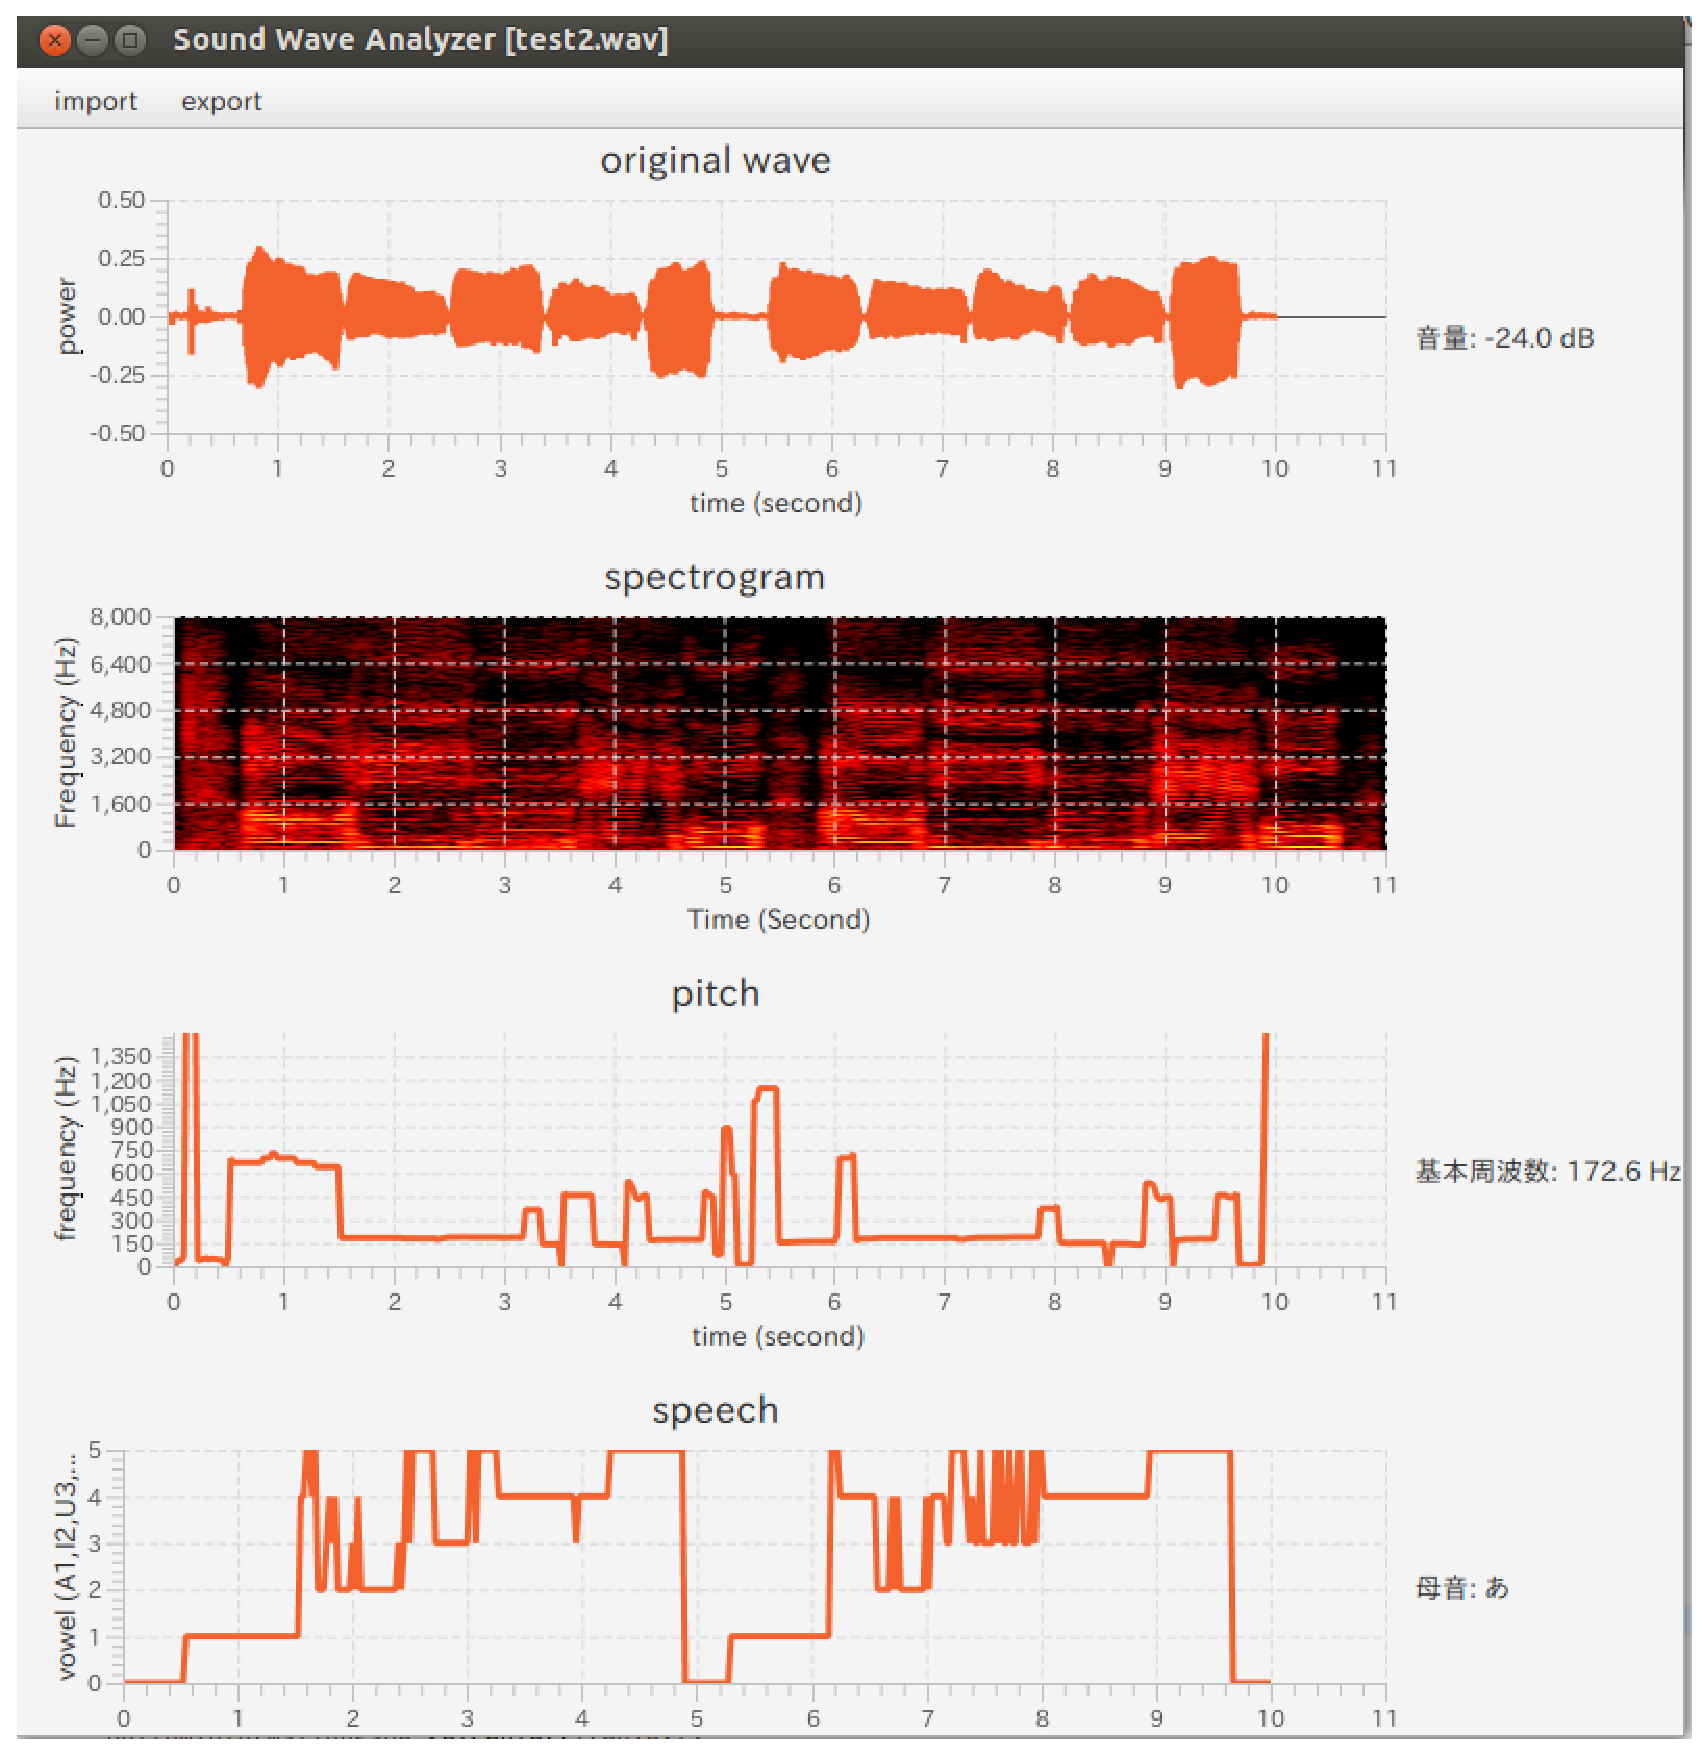
\includegraphics[scale=0.5]{gui.eps}
   \caption{GUI概観}
  \end{center}
\end{figure}


\subsection{クラス構成}
\begin{verbatim}
le4_music
 ┣ sound_wave_analyzer          …音響信号可視化GUI本体のパッケージ
 ┃ ┗ SoundWaveAnalyzer.java            …音響信号可視化GUIメインエントリ
 ┗ tools                        …音響解析やチャート表示に使用するツールパッケージ
    ┣ ChartTools.java                  …チャートの作成や操作を行うクラス
    ┣ Constants.java                   …解析ツールの定数の定義クラス
    ┣ ExportHandler.java               …画像ファイルへのエクスポートを行うクラス
    ┣ PlotLoudnessSimple.java          …音量解析のテストクラス
    ┣ PlotPitchSimple.java             …音高解析のテストクラス
    ┣ PlotRecognizedSpeech.java        …母音認識のテストクラス
    ┣ PlotSpectralEnvelopeSimple.java  …包絡抽出のテストクラス
    ┣ PlotSpectrogramSimple.java       …スペクトログラム解析のテストクラス
    ┣ PlotSpectrumSimple.java          …スペクトル解析のテストクラス
    ┣ PlotVoicedSound.java             …有声音抽出のテストクラス
    ┣ PlotWaveformSimple.java          …元波形表示のテストクラス
    ┣ SpeechRecognizer.java            …母音認識器のクラス
    ┗ TransformTools.java              …各種変換を行うクラス
\end{verbatim}


\section{機能詳細}

%%%%%%%%%%%%
\subsection{元波形表示機能}
入力された音響信号ファイルの波形をそのままGUI最上部に表示する。

\subsubsection{プログラム}
(元波形表示機能を担う重要部分を抜粋)
\begin{verbatim}
【tools.ChartTools.java】
…
/*
 * データからチャートを作成する
 */
public static LineChart<Number, Number> makeSimpleChart(
  double[] plotData,
  double xScale,
  String seriesName,
   String title,
   String xLabel,
   String yLable)
{
   // データ系列を作成
   final ObservableList<XYChart.Data<Number, Number>> data = 
     IntStream.range(0, plotData.length)
       .mapToObj(i -> new XYChart.Data<Number, Number>(i * xScale, plotData[i]))
       .collect(Collectors.toCollection(FXCollections::observableArrayList));

   // データ系列に名前をつける
      final XYChart.Series<Number, Number> series = new XYChart.Series<>();
      if(!seriesName.equals("")) series.setName(seriesName);
      series.setData(data);
   // 軸を作成
      final NumberAxis xAxis = new NumberAxis();
      xAxis.setLabel(xLabel);
      final NumberAxis yAxis = new NumberAxis();
      yAxis.setLabel(yLable);

   // チャート作成
      final LineChart<Number, Number> chart = new LineChart<>(xAxis, yAxis);
      chart.setTitle(title);
      chart.setCreateSymbols(false);
      chart.getData().add(series);
      return chart;
}
…

【sound_wave_analyzer.SoundWaveAnalyzer.java】
…
public void start(Stage primaryStage) throws Exception {
…
   // チャート作成
   LineChart<Number, Number> waveChart = ChartTools.makeSimpleChart(
      wave,
      1.0/sampleRate,
      "original wave",
      "time (second)",
      "power"
   );
…
}
…

\end{verbatim}

チャート作成はtools.ChartTools.javaクラスのstaticメソッド(makeSimpleChart)で行うようにした。
元波形については変形を行う必要がないので、.wavファイルから取得したdoubleの配列(wave)をそのまま渡した。
配列の要素1つがx軸方向のどれだけのスケールを占めるかを示す第2引数は、sampleRate(Hz)の逆数となる。

%%%%%%%%%%%%%%%
\subsubsection{テスト実行例}

元波形表示の機能だけをもつテストクラスtools.PlotWaveformSimple.javaで単体テストを行った。入力として、以下の2つの音響信号ファイルを使用した。\\
 \\
1. sample1.wav  繋げて発音された「あいうえお」\\
2. sample2.wav  短く発音された「あいうえお」\\
 \\
結果として以下の2つのチャートが得られた。

\begin{figure}[htbp]
 \begin{minipage}{0.5\hsize}
  \begin{center}
   \includegraphics[width=70mm]{wave1.eps}
  \end{center}
  \caption{sample1.wavの元波}
  \label{fig:one}
 \end{minipage}
 \begin{minipage}{0.5\hsize}
  \begin{center}
   \includegraphics[width=70mm]{wave2.eps}
  \end{center}
  \caption{sample2.wavの元波形}
  \label{fig:two}
 \end{minipage}
\end{figure}

sample1の波形には繋がった振動が、sample2の波形には短い時間の振動が5回確認できた。

以上より、元波形表示機能は期待された動作が確認された。

%%%%%%%%%%%%%%
\subsection{スペクトログラム表示機能}
入力された音響信号ファイルのスペクトログラムを上から2段目に表示する。
スペクトログラムデータの計算には、短時間フーリエ変換を用いた。

\subsubsection{プログラム}
(スペクトログラム機能を担う重要部分を抜粋)
\begin{verbatim}
【tools.TransformTools.java】
…
/*
 * 音波(width-time)をスペクトログラム(dB-(Hz-time))に変換
 */
public static double[][] toSpectrogram(
   double[] wave,
   int frameSize,
   int shiftSize)
{
   // 2^pとなる配列サイズを求める
   final int fftSize = 1 << Le4MusicUtils.nextPow2(frameSize);

   // 窓関数と正規化
   final double[] window = MathArrays.normalizeArray(
      Arrays.copyOf(Le4MusicUtils.hanning(frameSize),fftSize),
         1.0
   );

   // 短時間フーリエ変換
   final Stream<Complex[]> spectrogram = 
      Le4MusicUtils.sliding(wave, window, shiftSize)
         .map(frame -> Le4MusicUtils.rfft(frame));
         // デシベル化
   return spectrogram.map(sp -> 
         Arrays.stream(sp).mapToDouble(c -> toDB(c.abs())).toArray()
      ).toArray(n -> new double[n][]);
}
…


【tools.PlotSpectrogramSimple.java】
…
/*
 * スペクトログラム用のチャートを作成する
 */
public static LineChartWithSpectrogram<Number, Number> makeSpectrogramChart(
   double[][] spectrogramData,
   double frameDuration,
   double shiftDuration,
   double sampleRate,
   String title,
   String xLabel,
   String yLabel)
{
   // 窓関数のフレーム長 // s * 1/s
   final int frameSize = (int) Math.round(frameDuration * sampleRate);
   // 何要素分シフトするか
   final int shiftSize = (int) Math.round(shiftDuration * sampleRate);

   // 2^pとなる配列サイズを求める
   final int fftSize = 1 << Le4MusicUtils.nextPow2(frameSize);
   final int fftHalfSize = (fftSize >> 1) + 1;
		
   // x軸
   final NumberAxis xAxis = new NumberAxis();
   xAxis.setLabel("Time (Second)");
   xAxis.setLowerBound(0.0);
   xAxis.setUpperBound(spectrogramData.length * shiftDuration);
   // y軸
   final NumberAxis yAxis = new NumberAxis();
   yAxis.setLabel("Frequency (Hz)");
   yAxis.setLowerBound(0.0);
   yAxis.setUpperBound(sampleRate * 0.5);
   yAxis.setTickUnit(sampleRate * 0.05);
   yAxis.setAutoRanging(false);
		
   // チャート作成
   final LineChartWithSpectrogram<Number, Number> chart = new LineChartWithSpectrogram<>(xAxis, yAxis);
   chart.setParameters(spectrogramData.length, fftHalfSize, sampleRate * 0.5);
   chart.setTitle(title);
   Arrays.stream(spectrogramData).forEach(chart::addSpecLog);
   chart.setCreateSymbols(false);
   chart.setLegendVisible(false);
		
   return chart;
}


【sound_wave_analyzer.SoundWaveAnalyzer.java】
…
@Override
public void start(Stage primaryStage) throws Exception {
…
   // 波形変換
   double[][] spectrogram = TransformTools.toSpectrogram(wave, frameSize, shiftSize);
…
   //チャートを作成
   LineChartWithSpectrogram<Number,Number> spectrogramChart 
      = PlotSpectrogramSimple.makeSpectrogramChart(
         spectrogram, 
         frameDuration, 
         shiftDuration, 
         sampleRate, 
         "spectrogram", 
         "time (second)",
         "frequency (Hz)"
   );
   ChartTools.setYAxisDetails(spectrogramChart, sampleRate*0.5, sampleRate*0.1);
…
\end{verbatim}
\subsubsection{テスト実行例}

スペクトログラム表示の機能だけをもつテストクラスtools.PlotSpectrogramSimple.javaで単体テストを行った。入力として、以下の3つの音響信号ファイルを使用した。\\
 \\
1. sample1.wav  繋げて発音された「あいうえお」\\
2. sample2.wav   短く発音された「あいうえお」\\
3. sample3.wav    低い音→高い音→低い音と連続的に変化させた音声\\
 \\
結果として以下の3つのチャートが得られた。

\begin{figure}[htbp]
 \begin{minipage}{0.5\hsize}
  \begin{center}
   \includegraphics[width=70mm]{spec1.eps}
  \end{center}
  \caption{sample1.wavのスペクトログラム}
  \label{fig:one}
 \end{minipage}
 \begin{minipage}{0.5\hsize}
  \begin{center}
   \includegraphics[width=70mm]{spec2.eps}
  \end{center}
  \caption{sample2.wavのスペクトログラム}
  \label{fig:two}
 \end{minipage}
\end{figure}

\begin{figure}[htbp]
 \begin{minipage}{0.5\hsize}
  \begin{center}
   \includegraphics[width=70mm]{spec3.eps}
  \end{center}
  \caption{sample3.wavのスペクトログラム}
  \label{fig:one}
 \end{minipage}
\end{figure}

sample1のスペクトログラムには、時間的に連続的な、5種類のはしごのような模様が確認できた。
sample2のものには、時間的に切れた、5種類の幅の短いはしご模様が確認できた。
sample3のものには、連続的な山のような模様が確認できた。

以上より、スペクトログラム表示機能には期待された動作が確認された。

\subsection{基本周波数(音高)表示機能}
入力された音響信号ファイルの基本周波数のグラフを上から3段目に表示する。
基本周波数は、自己相関の第2極大値として算出した。
\subsubsection{プログラム}
(スペクトログラム機能を担う重要部分を抜粋)
\begin{verbatim}
【tools.TransformTools.java】
…
/*
 * 短時間音波を音高(Hz)に変換
 * (基本周波数の抽出)
 */
public static double getPitch(
   double[] miniWave,
   double sampleRate) 
{
   int phase = 0;
   int maxSlide = 0;
   double max = 0;
   for(int i=0;i<miniWave.length;i++) {
      double sum = 0;
      for(int j=0;j<miniWave.length-i;j++) {
         sum += miniWave[j]*miniWave[j+i]; // 自己相関を計算
      }
     
      if(phase == 0) { // 第一の山
         if(sum < 0) phase = 1;
      }else if(phase == 1) { // 第一の谷
         if(sum > 0) phase = 2;
      }else {
         if(sum > max) {
            maxSlide = i;
            max = sum;
         }
         if(sum < 0) break;
      }
   }
   if(maxSlide == 0) return 0;
   return sampleRate / maxSlide;
}
	
/*
 * 音波を音高(Hz)の列に変換
 */
public static double[] toPitch(
   double[] wave,
   double sampleRate,
   int frameSize,
   int shiftSize)
{
   double[] pitch = 
      Le4MusicUtils.sliding(wave, frameSize , shiftSize).mapToDouble(
      frame -> getPitch(frame,sampleRate)).toArray();
   return pitch;
}
…

【sound_wave_analyzer.SoundWaveAnalyzer.java】
…
@Override
   public void start(Stage primaryStage) throws Exception {
…
   //波形変換
   double[] pitch = TransformTools.toPitch(wave, sampleRate, frameSize, shiftSize);
…
   //チャート作成
   LineChart<Number, Number> pitchChart = ChartTools.makeSimpleChart(
      pitch,
      shiftDuration,
      "pitch",
      "time (second)",
      "frequency (Hz)"
   );
   ChartTools.setYAxisDetails(pitchChart, 1500,150);
…
\end{verbatim}
\subsubsection{テスト実行例}
基本周波数表示の機能だけをもつテストクラスtools.PlotPitchSimple.javaで単体テストを行った。入力として、以下の2つの音響信号ファイルを使用した。\\
 \\
1. C.wav      ピアノのC4(約261.63Hz)\\
2. oshirase.wav   1-3-5-8-10-8-5-3-1 の音高で推移する連続した声音\\
 \\
結果として以下の2つのチャートが得られた。

\begin{figure}[htbp]
 \begin{minipage}{0.5\hsize}
  \begin{center}
   \includegraphics[width=70mm]{pitchC.eps}
  \end{center}
  \caption{C.wavの基本周波数}
  \label{fig:one}
 \end{minipage}
 \begin{minipage}{0.5\hsize}
  \begin{center}
   \includegraphics[width=70mm]{oshirasePitch.eps}
  \end{center}
  \caption{oshirase.wavの基本周波数}
  \label{fig:two}
 \end{minipage}
\end{figure}

C.wavには、261Hzから264Hz周辺に一直線なグラフが確認できた。
oshirase.wavには、階段状に推移するグラフが確認できた。

以上より、基本周波数表示機能には期待された動作が確認された。

\subsection{母音識別機能}
入力された音響信号ファイルの母音識別結果を最下段に表示する。

母音識別は、tools.SpeechRecognizerクラスをメインエントリとする教師データ作成機能と、同クラスのインスタンスを識別器とする認識機能の2つの機能から成る。

教師データ作成機能は、「あ」「い」「う」「え」「お」の5つの音声ファイルを入力とし、それぞれの音声の13次元ケプストラムベクトルの平均・分散の情報が記述された教師ファイル(vowel.tch)を出力する。

認識機能は、音響信号ファイルを入力として、教師ファイルを用いた正規分布に従う認識を行った結果をグラフとして出力する(あ-1,い-2,う-3,え-4,お-5)。有声音認識と音量認識によるフィルターをかけ、より認識が正確となるようにしている。

\subsubsection{教師データ作成機能のプログラム}
\begin{verbatim}
【tools.SpeechRecognizer.java】
…
/*
 * 教師ファイルを作成(.wav -> vowel.tch)
 */
public static void main(String[] args) {
   if(args.length != 5) {
      System.out.println("please give 5 teacher wav files - A,I,U,E,O");
      return;
   }
   double[][] teacherDatas = new double[10][Constants.CEPSTRUM_DIMENSION];
   try {
      // AIUEOそれぞれのファイルで学習
      for(int i=0; i<5; i++) {
         System.out.print("...file("+(i+1)+"): ");
         
         // wavファイル読み込み
         File wavFile = new File(args[i]);
         AudioInputStream stream = AudioSystem.getAudioInputStream(wavFile);
         double[] wave = Le4MusicUtils.readWaveformMonaural(stream);
         AudioFormat format = stream.getFormat();
         double sampleRate = format.getSampleRate();
         stream.close();
			
         double frameDuration = Le4MusicUtils.frameDuration;
         double shiftDuration = frameDuration / 8.0;
         int frameSize = (int) Math.round(frameDuration * sampleRate);
         int shiftSize = (int) Math.round(shiftDuration * sampleRate);
			
         // ケプストラム抽出
         ArrayList<double[]> cepstrum = new ArrayList<>();
         Le4MusicUtils.sliding(wave, frameSize , shiftSize).forEach(
            frame -> {
              // 有声音のデータだけ抽出
          if(TransformTools.isVoicedSound(wave, sampleRate)) {
            double[] ceps = TransformTools.getCepstrum(frame);
            if(!Double.isInfinite(ceps[0])) cepstrum.add(ceps);
          }
        }
      );
      // データの平均を計算
      double[] mean = new double[Constants.CEPSTRUM_DIMENSION];
      for(int k=0; k<cepstrum.size(); k++) {
         double[] ceps = cepstrum.get(k);
         for(int j=0;j<ceps.length;j++) {
            mean[j] += ceps[j]/cepstrum.size();
            }
      }			
      //データの分散を計算
      double[] dispersion = new double[Constants.CEPSTRUM_DIMENSION];
      for(int k=0; k<cepstrum.size(); k++) {
            double[] ceps = cepstrum.get(k);
            for(int j=0;j<ceps.length;j++) {
               dispersion[j] += Math.pow((ceps[j]-mean[j]),2)/cepstrum.size();
            }
         }
         teacherDatas[i*2] = mean;
         teacherDatas[i*2+1] = dispersion;
         System.out.println("complete");
      }
			
      // データを書き込み
      BufferedWriter out = new BufferedWriter(
      new FileWriter(new File(Constants.SPEECH_RECOGNITION_TEACHER_FILE)));
      for(int i=0;i<teacherDatas.length; i++) {
         double[] data = teacherDatas[i];
         for(int j=0; j<data.length; j++) {
            out.write(data[j]+" ");
         }
         out.newLine();
      }
			
      out.close();
      System.out.println("finish.");
   }catch(Exception e) {
      e.printStackTrace();
      System.out.println("File reading error!");
   }
}
…
\end{verbatim}
\subsubsection{認識機能のプログラム}
\begin{verbatim}
【tools.SpeechRecognizer.java】
…
/*
 * 音声認識器の作成
 */
public SpeechRecognizer() {this(Constants.SPEECH_RECOGNITION_TEACHER_FILE);}
   public SpeechRecognizer(String teacherFile) {
    // 認識モデル読み込み(vowel.tch -> data)
    mean = new double[6][Constants.CEPSTRUM_DIMENSION];
    dispersion = new double[6][Constants.CEPSTRUM_DIMENSION];
     try {
         BufferedReader in = new BufferedReader(
            new FileReader(new File(teacherFile)));
      for(int i=1;i<=5;i++) {
         double[] valuesM = Arrays.stream(in.readLine().trim().split(" "))
            .mapToDouble(v -> Double.valueOf(v))
            .toArray();
         double[] valuesD = Arrays.stream(in.readLine().trim().split(" "))
            .mapToDouble(v -> Double.valueOf(v))
            .toArray();
         if(valuesM.length == Constants.CEPSTRUM_DIMENSION
               && valuesD.length == Constants.CEPSTRUM_DIMENSION) {
            mean[i] = valuesM;
            dispersion[i] = valuesD;
         }else {
            in.close();
            throw new Exception("data dimension must be "
               +Constants.CEPSTRUM_DIMENSION);
         }
      }
      in.close();
      prepared = true;
    }catch(Exception e) {
      e.printStackTrace();
      System.out.println("file read error!");
    }
}
	
/*
 * 短時間の音波を音声認識する
 * @return 母音を表す整数(SpeechRecognizer.A,I,U,E,O)
 */
public double recognize(double[] miniWave) {
   if(!prepared) {
   System.out.println("SpeechRecognizer is NOT prepared!");
      return 0;
   }
   double[] cepstrum = TransformTools.getCepstrum(miniWave);
   double max = Double.NEGATIVE_INFINITY;
   double maxVowel = 0;
   double likelihood = calcLikelihood(cepstrum,A);
   if(likelihood > max) {
      max = likelihood;
      maxVowel = A;
   }
   …
   likelihood = calcLikelihood(cepstrum,O);
   if(likelihood > max) {
      max = likelihood;
      maxVowel = O;
   }
   return maxVowel;
 }
	
/*
 * 音波を母音の列に変換
 */
public double[] toSpeach(
   double[] wave, 
   double sampleRate, 
   int frameSize, 
   int shiftSize) 
{
   double[] speach = 
   Le4MusicUtils.sliding(wave, frameSize , shiftSize).mapToDouble(frame ->
      // 無声音,雑音は0とする
      (TransformTools.isVoicedSound(frame, sampleRate) &&
            TransformTools.getRMSdB(frame)>Constants.LOUDNESS_FILTER)? 
         recognize(frame):
         0
      ).toArray();
   return speach;
}
	
/*
 * 母音に対する特徴ベクトルの尤度を計算
 */
private double calcLikelihood(double[] cepstrum, int vowel) {
   if(vowel != A && vowel != I &&vowel != U &&vowel != E &&vowel != O) {
      return 0;
   }
   return calcNomalDistribution(cepstrum, mean[vowel], dispersion[vowel]);
}
	
/*
 * 正規分布(簡易)の確率密度関数から値を算出
 */
private double calcNomalDistribution(
   double[] x, double[] mean, double[] dispersion) {
		
   double logsum = 0;
   for (int i = 0; i < mean.length; i++) {
      logsum -= Math.log(Math.sqrt(dispersion[i]))
         +Math.pow(x[i]-mean[i], 2)/(2*dispersion[i]);
   }
   return logsum;
}

【sound_wave_analyzer.SoundWaveAnalyzer.java】
…
@Override
public void start(Stage primaryStage) throws Exception {
…
   //識別器の作成
   SpeechRecognizer recognizer = new SpeechRecognizer();
   …
   //波形変換
   double[] speech = recognizer.toSpeach(wave, sampleRate, frameSize, shiftSize);
   …
   //チャートの作成
   LineChart<Number, Number> speechChart = ChartTools.makeSimpleChart(
      speech,
      shiftDuration,
      "speech",
      "time (second)",
      "vowel (A1,I2,U3,E4,O5)"
   );
   ChartTools.setYAxisDetails(speechChart, 5.0, 1.0);
…
}
\end{verbatim}
\subsubsection{テスト実行例}
まず、以下の5つの音声ファイルを入力としてtools.SpeechRecognizer.javaを動作させ、教師ファイル(vowel.tch)を作成した。\\
 \\
1. teacherA.wav 「あー」と5秒間発音した音声ファイル\\
2. teacherI.wav 「いー」と5秒間発音した音声ファイル\\
3. teacherU.wav 「うー」と5秒間発音した音声ファイル\\
4. teacherE.wav 「えー」と5秒間発音した音声ファイル\\
5. teacherO.wav 「おー」と5秒間発音した音声ファイル\\

次に、母音識別の機能だけをもつテストクラスtools.PlotRecognizedSpeech.javaで単体テストを行った。入力として、以下の2つの音響信号ファイルを使用した。\\
 \\
1. aiueoaiueo.wav        「あいうえお」を二回発音した音声\\
2. korehatesutodayo.wav   「これはテストだよ」と発音した音声\\
 \\
結果として以下の2つのチャートが得られた。

\begin{figure}[htbp]
 \begin{minipage}{0.5\hsize}
  \begin{center}
   \includegraphics[width=70mm]{aiueoaiueo.eps}
  \end{center}
  \caption{aiueoaiueo.wavの母音判定結果}
  \label{fig:one}
 \end{minipage}
 \begin{minipage}{0.5\hsize}
  \begin{center}
   \includegraphics[width=70mm]{korehatesutodayo.eps}
  \end{center}
  \caption{korehatesutodayo.wavの母音判定結果}
  \label{fig:two}
 \end{minipage}
\end{figure}


aiueoaiueo.wavについては、期待した出力「1234512345」に近い階段状のグラフが確認できた。
korehatesutodayo.wavについては、期待した出力「54143515」に近い形状のグラフが確認できた。
「あ」「え」「お」の認識が比較的うまくいっている一方で、「い」は「え」に、「う」は「お」に引っ張られる傾向が見られた。

いずれの入力の場合も、一部結果がブレている箇所が確認されたので、今後はより質の良い教師データの生成や、より精度の高い認識方法を試していきたい。

精度には改善の余地があるが、以上より母音認識機能の正しい動作が確認された。

\end{document}


%%%%%%%%%%%%%%%%%%%%%%%%%%%%%%%%%%%%%%%%%%%%%%%%%%%%%% 以下参考

\section{セクション}
内容

段落改行は一行あける
\subsection{サブセクション}
\subsection{サブセクション}

\subsection{箇条書き}
\begin{description}
\item [表題]~\\
内容はここに書く
\item[表題]\mbox{}\\
内容はここに書く
\item[表題に括弧を使う$<$括弧$>$]
\end{description}

\subsection{箇条書き(番号付き)}
\begin{enumerate}
\item 表題 ~\\
内容はここに書く 
\item 表題 \mbox{}\\
内容はここに書く 
\end{enumerate}

\subsection{図の挿入}
% 図のファイル名,拡大縮小率を調整する.
%\begin{center}
%  \includegraphics[scale=0.65]{figure01.eps}
%\end{center}

\subsection{スクリーン}
\begin{screen}
~\\
単純改行\\
$【括弧】$\\
$<括弧>$ \\
\end{screen}
\begin{verbatim}
文書挿入
\end{verbatim}
